\normalfalse \difficilefalse \tdifficiletrue
\correctionfalse

%\UPSTIidClasse{11} % 11 sup, 12 spé
%\newcommand{\UPSTIidClasse}{12}

\exer{Système EPAS $\star$ \label{C2:06:64}}

\setcounter{question}{0}\UPSTIcompetence[2]{C2-06}
\index{Compétence C2-06}
\index{EPAS}
\ifcorrection
\else
\textbf{Pas de corrigé pour cet exercice.}
\fi



\ifprof
\else
Nous allons déterminer la vitesse de sortie des vérins pour que la vitesse des points de la
plate-forme soit constante.

On propose le paramétrage suivant : 
\begin{itemize}
\item le repère $\rep{0}=\repere{O_0}{x_0}{y_0}{z_0}$ est lié au châssis (0);
\item le repère $\rep{5}=\repere{A}{x_5}{y_5}{z_0}$ est lié à l’ensemble \{berceau+parc échelle\} (5) avec 
$\vect{O_0 A}=a\vect{y_0}$ et $\couple{x_0}{x_5}=\theta$, $\vect{AC}=c\vect{x_5}$, $\vect{AD}=H\vect{x_5}$;
\item le repère $\rep{3}=\repere{B}{x_3}{y_3}{z_0}$ est lié au vérin (3+4) avec $\vect{O_0 B}=b\vect{x_0}$ et $\vect{BC}=r\vect{y_3}$ et $\beta = \couple{x_0}{x_3}$.
\end{itemize}

\begin{center}
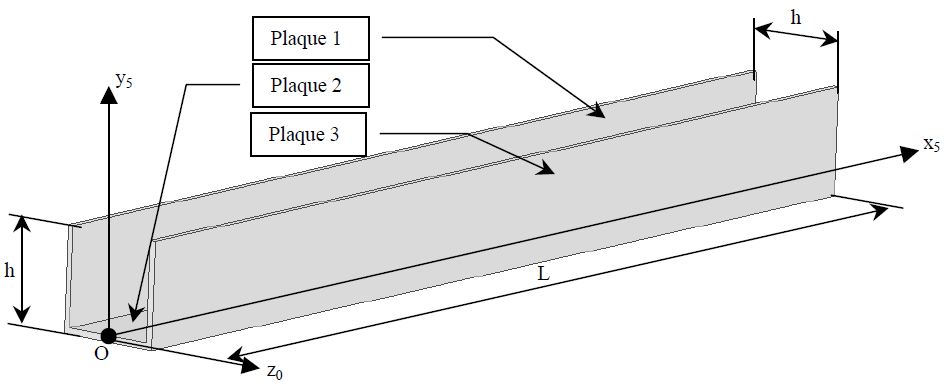
\includegraphics[width=\linewidth]{64_01}
\end{center}
\fi

\question{Tracer le graphe des liaisons.}
\ifprof
\else
\fi

\question{Exprimer la vitesse du point $D$ du parc échelle dans son mouvement par rapport
au châssis : $\vectv{D}{5}{0}$ en fonction de la vitesse angulaire de dressage $\dot{\theta}$ et des paramètres
géométriques.}
\ifprof
\else
\fi

\question{En faisant une fermeture de chaîne cinématique, déterminez la vitesse de sortie du vérin 
$\vectv{V}{4}{3} = v\vect{y_3}$ en fonction de la vitesse angulaire de dressage et des paramètres
géométriques.}
\ifprof
\else
\fi

\question{Etablir la relation $\tan\beta = \dfrac{b-c \cos \theta}{a+c\sin\theta}$ en écrivant une fermeture de chaîne
géométrique.}
\ifprof
\else
\fi


\question{Déduire des questions précédentes la vitesse de sortie des vérins $v$ en fonction de
$\theta$ et $H$ et des constantes $a$, $b$, $c$ ; pour que la vitesse du point $D$ du parc échelle soit constante.}
\ifprof
\else
\fi



\ifprof
\else
\footnotesize
Eléments de corrigé : 
\begin{itemize}
\item .
\item $\vectv{D}{5}{0} =H\dot{\theta}\vect{y_5}$.
\item $v=c\dot{\theta}\cos\left(\theta-\beta \right)$.
\item $v=\dot{r}=\dfrac{c\dot{\theta}\left(a\cos\theta+b\sin\theta\right)}{\sqrt{\left(b-c\cos\theta \right)^2+\left(a+c\sin\theta \right)^2+}}$.
\end{itemize}
\normalsize
\begin{flushright}
\footnotesize{Corrigé  voir \ref{C2:06:64}.}
\end{flushright}%
\fi